\documentclass{article}
\usepackage{tikz}
\tikzset{help lines/.style=very thin}
\tikzset{Karl's grid/.style={help lines, color=#1!50},
         Karl's grid/.default=blue}
\begin{document}
We are working on
  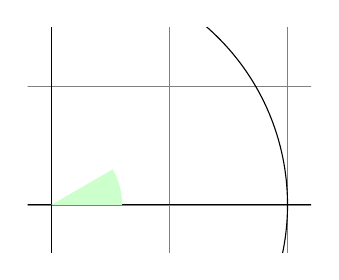
\begin{tikzpicture}[scale=3]
    %\draw[Karl's grid=red] (0,0) grid (5,5);
    \clip (-0.1,-0.2) rectangle (1.1, 0.75);
    \draw[step=0.5cm, gray, very thin] (-1.4,-1.4) grid (1.4,1.4);
    \draw (-1.5,0)--(1.5,0);
    \draw (0,-1.5)--(0,1.5); %Now add the half circle
    \draw (0,0) circle [radius=1cm];
    \fill[green!20!white] (0,0)--(3mm,0mm)
      arc [start angle=0, end angle=30, radius=3mm]--cycle;
  \end{tikzpicture}

Curved Path Construction.
  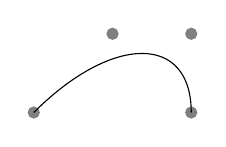
\begin{tikzpicture}
    \filldraw[gray] (0,0) circle [radius=2pt]
                    (1,1) circle [radius=2pt]
                    (2,1) circle [radius=2pt]
                    (2,0) circle [radius=2pt];
    \draw (0,0) .. controls (1,1) and (2,1) .. (2,0);
  \end{tikzpicture}
  \tikz \draw (0,0) circle [radius=10pt];
  \tikz \draw[rotate=30] (0,0) ellipse [x radius=20pt,y radius=10pt];
  \tikz \draw[x=1.57ex,y=1ex] (0,0) sin (1,1) cos (2,0) sin (3,-1) cos (4,0)
                              (0,1) cos (1,0) sin (2,-1) cos (3,0) sin (4,1);
\end{document}
